\chapter{拓扑物态的深度学习} \label{chap:topoml}

这一章,我们讨论拓扑物态的机器学习问题。首先,我们在第 \ref{sec:classify} 小节介绍拓扑物态分类的一般性理论,特别的,我们将介绍到一维 AIII 类的对称性约束与拓扑刻画,以及二维 A 类 的对称性及拓扑刻画理论;在 \ref{sec:neuralnetwork} 节,我们介绍一种机器学习的算法,人造神经网络结构;在 \ref{sec:topoml} 我们讨论利用深度神经网络进行拓扑物态的机器学习问题,我们将介绍对于一维 AIII 类 四能带模型 的 绕数的学习,以及二维 A类 二能带模型的 Chern 数的学习。



\section{拓扑物态分类通论} \label{sec:classify}
在第 \ref{chap:chargepump} 章中,我们讨论了一类有能隙的费米子体系的绝热周期性演化,其绝热周期幺正演化算符最终会与某类 一维系统上定义的 绕数(winding number)和二维参数空间上定义的陈数(Chern number)相联系。这些拓扑数表征了体系在某些方面的性质上具有量子化的整数平台,在前面的电荷输运的例子中,表现为系统每周期输运整数倍的电荷单位。这其实就是一个拓扑物态的例子。正如前文所述,拓扑物态的诸多良好性质,如鲁棒性、量子化平台等,吸引人们在过去几十年间对其进行了大量的研究。人们通过对大量特殊模型的研究,渐渐建立起了一套系统性的拓扑物态的分类理论\cite{topoclassify2016},下面进行介绍。

拓扑绝缘体讨论有能隙的无相互作用作用费米子体系。根据体系所具有的对称性的不同,可划分为一下十类:A,AIII,AI,BDI,D,DIII,AII,CII,C,和 CI 类。对于不同类(也就是不同对称性)的模型,可以用不同的拓扑数来刻画,其拓扑刻画的规律随着体系维度的变化而变化。对某一类维度和对称性的模型,其完整的拓扑刻画可能对应到例如 $\mathbb{Z}$,$2\mathbb{Z}$,或 $\mathbb{Z}_2$,甚至0。根据对称性的变化和模型维度的变化,人们建立起一个周期表(Periodic Table)来描述不同类别模型拓扑刻画的规则(叫\textit{周期表}是因为随着体系维度增加呈现出周期性结构),具体可参考文献\inlinecite{topoclassify2016}。我们这里具体讨论两类,一维 AIII 类 和二维 A 类,这两类也是后面 \ref{sec:topoml} 节我们展开机器学习的类别。

在具体介绍 A 类 和 AIII 类之前,先让我们回顾第 \ref{chap:dynm} 章中提到的几种对称性变换。
\begin{itemize}
    \item 时间反演变换 $\mathcal{T}$:为反幺正变换,将 $\ii$ 映射为 $-\ii$
    \begin{align}
    \mathcal{T} \ii \mathcal{T}^{-1} \rightarrow \ii
    \end{align}

    \item 粒子空穴变换 $\mathcal{C}$:幺正变换,将费米子湮灭算符 $\psi$ 映射为产生算符 
    \begin{align}
        \mathcal{C}\psi\mathcal{C}^{-1} \rightarrow \psi^{\dag}
    \end{align}

    \item 手征变换,为时间反演变换和粒子空穴变换的结合,
    \footnote{在第 \ref{chap:dynm} 章中,时间反演算符和粒子空穴变换的记号分别为 $R$,$\mathcal{P}$,而 $S$ 用来指代时间反演变换和另一个幺正变换 $W$ 所结合的反幺正变换。}
    \begin{align}
        \mathcal{S} = \mathcal{T} \mathcal{C}
    \end{align}

\end{itemize}
根据是否具有这几种对称性,无相互作用的费米子体系被划分为上述10类。
其中,
A 类是一般的无特殊对称性约束的体系,只有在偶数维度的体系($d=2n$)中具有非平庸的拓扑分类,由 Chern 数刻画:
\begin{align}
C_n = \frac{1}{n!}\left(\frac{1}{2\pi}\right)^{n}\int\text{Tr} F^n
\end{align}
其中 
\begin{align}
F = dA - \ii A^2
\end{align}
$A$ 为被填充能带的 非阿贝尔联络,
定义如下
\begin{align}
A_i^{mn} = A_i^{mn}dk^i = \ii \langle u^m(\vect{k})|\partial_{\vect{k}_i} u^n(\vect{k})\rangle
\end{align}
类似于 第\ref{chap:chargepump} 章中 提到的非阿贝尔 Berry 联络,只是这里使用了微分的记号。$n=1$ 时就是由第一 Chern 数所刻画的二维模型,著名的例子如 Haldane 模型\cite{haldane1988} 就是一种 Chern 类绝缘体。对于这一 Chern 数,我们在附录 \ref{sec:chern} 中讨论了基于 \inlinecite{chern2005} 的算法,并证明了其相关性质。


而 AIII 类是只具有上述手征对称性($\mathcal{S}$)的体系。例如,第 \ref{chap:chargepump} 章中提到的 SSH 模型,即一维 AIII 类模型。由于手征对称性由粒子空穴对称性和时间反演对称性组合而成,粒子空穴对称性会将费米子产生算符映射为湮灭算符,因此,能谱须正负对称\footnote{迹不为0的情况相当于加了一常数矩阵,将其拿掉后还是正负对称},具有该对称性的哈密顿量矩阵 $\mathcal{H}(\vect{k})$,
\footnote{哈密顿量是 $H$,哈密顿量矩阵是 $\mathcal{H}(\vect{k})$}
\begin{align}
H(\vect{k}) = \psi_{\vect{k}}^{\dag}\mathcal{H}(\vect{k})\psi_{\vect{k}}
\end{align}
能找到幺正矩阵 $\mathcal{U}_S$ 与之反对易。
\begin{align}
\{\mathcal{U}_S, \mathcal{H}(\vect{k})\} = 0
\end{align}
以上要求保证了在 $\mathcal{U}_S$ 对角的基矢下,哈密顿量矩阵可写作如下块矩阵形式
\begin{align}
\mathcal{H}(\vect{k}) = \begin{pmatrix}
0 & D(\vect{k}) \\
D(\vect{k})^{\dagger} & 0
\end{pmatrix}
\end{align}
其中,$D(\vect{k})$ 幺正。
例如,这里再次举 SSH 的例子。SSH 哈密顿量在时空间写作
\begin{align}
H = -\sum_jt_1a^{\dagger}_{j}b_{j} + t_2 b^{\dagger}_ja^{j+1}_{j+1} + \text{H.c.}
\end{align}
变换到 $\vect{k}$-空间,哈密顿量写作
\begin{align}
H = \sum_{\vect{k}}
\begin{pmatrix}
a_{\vect{k}}^{\dag} & b_{\vect{k}}^{\dag}
\end{pmatrix}
\begin{pmatrix}
0 & t_1 + t_2e^{-\ii\vect{k}} \\
t_1 + t_2e^{\ii\vect{k}} & 0
\end{pmatrix}
\begin{pmatrix}
a_{\vect{k}} \\ b_{\vect{k}}
\end{pmatrix}
\end{align}
哈密顿量矩阵为
\begin{align}
\mathcal{H}(\vect{k}) = 
\begin{pmatrix}
0 & t_1 + t_2e^{-\ii\vect{k}} \\
t_1 + t_2e^{\ii\vect{k}} & 0
\end{pmatrix}
\end{align}
而这里找到的幺正矩阵为 $\hat{\mathcal{U}}_S = \sum_{\vect{k}} a^{\dag}_{\vect{k}}a_{\vect{k}} - b^{\dag}_{\vect{k}}b_{\vect{k}} $,
\begin{align}
\mathcal{U}_S = \begin{pmatrix}
1 & 0 \\
0 & -1 
\end{pmatrix} 
= \sigma_z
\end{align}
由于有上述形式的约束,对 AIII 类的刻画等价于对 $D(\vect{k})$ 的刻画。人们发现,只有在奇数维度的体系($d=2n+1$)才存在非平庸的拓扑分类,由绕数刻画,
\begin{align}
v_n = \dfrac{(-1)^nn!}{(2n+1)!}\left(\dfrac{\ii}{2\pi}\right)^{n+1}
\int\text{Tr}[(D^{-1}dD)^{2n+1}]
\end{align}
$d=1$, $n=0$ 时为一维的例子,由
\begin{align}
v_1 = \frac{\ii}{2\pi}\int_{\text{BZ}}\text{Tr}[D^{-1}dD]
\end{align}
刻画。例如上面提到的 SSH 模型,$t_1>t_2$ 时 $v_1=0$,$t_1<t_2$ 时 $v_1=1$。



\section{神经网络算法简介} \label{sec:neuralnetwork}
神经网络的算法结构经由 Geoffrey Hinton 等人的发展现在已经是机器学习中常用的成熟算法。神经网络在选择合适的激活元的情况下可以进行逆向传播
\footnote{逆向传播,backpropagation,其数学最早由 Yann LeCun 证明}
的过程,因此可以进行\textit{学习}。
特别是后来 Geoffrey Hinton 等人提出 Dropout 等方法,使该算法在许多特定的任务上表现出色,例如 ImageNet 做图像识别\cite{imagenet2012}。对该算法的详细的讨论可参见\cite{prmlbook}。这里不再赘述。这里只对两种特殊的神经结构做描述,一种是全连接神经网络层,一种是卷积神经网络层\footnote{也由 Yann LeCun 最早提出}。

\begin{figure}[t]
\centering
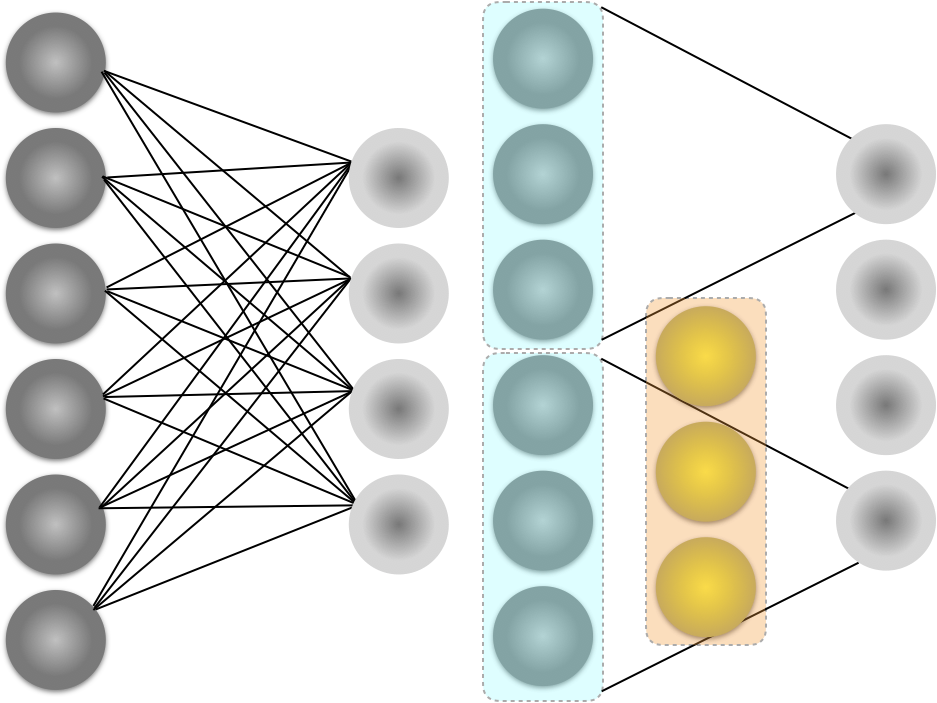
\includegraphics[width=1.0\columnwidth]{chap5_ml/neuralnetwork}
\caption{神经网络层示意图。左:全连接神经网络层。右:卷积神经网络层,中间的黄色块表示卷积核。}
\label{fig:nn}
\end{figure}


\subsection{全连接神经网络}
全连接神经网络层的结构如图 \ref{fig:nn}(左) 所示。其数学定义如下:
\begin{align}
y_i = (f_{\text{F.C.}}(\vecr{x}))_i = f(a_{ij}x_j + b_i)
\end{align}
这里的 $\vecr{x}$ 对应图中左栏的输入,$x_j$ 是左栏输入中的第 $j$ 个元素,$y_i$ 对应右栏的输出中的第 $i$ 元素。这其实就是一个线性变换,图中从左栏连接右栏的一组实线代表了该线性变换的矩阵。$f$ 函数是一个非线性函数
\footnote{$f$ 是非线性函数非常重要,否则一系列线性变换接起来还是线性变换,将无法拟合非线性函数。}
,也叫激活元,一般取 sigmoid 函数或 ReLU 函数或其变形 \cite{prmlbook,topoml} ,sigmoid 函数也就是 tanh 函数,ReLU 函数定义如下
\begin{align}
f(x) = \begin{cases}
0, & x\leq0 \\
x, & x>0
\end{cases}
\end{align}

一系列全连接神经网络层相接得到的神经网络结构为
\begin{align}
f_{\text{F.C.}}^n\circ f_{\text{F.C.}}^{n-1}\circ \cdot f_{\text{F.C.}}^1\circ(\vecr{x})
\end{align}
其中引入了如下定义
\begin{align}
f_{\text{F.C.}}^{n}\circ f_{\text{F.C.}}^{n-1}(\vecr{x})
= f(a^{n}_{ij}[f(a^{n-1}_{jk}x_k + b^{n-1}_j)]_{j} + b^n_i)
\end{align}

这就是全连接神经网络层的构造方式,全连接(Fully-Connected)的含义就是输入层的每一个元素都连接到输出层的每一个元素,通过线性变换和非线性变换。




\subsection{卷积神经网络}
卷积神经网络层的结构如图 \ref{fig:nn}(右) 所示。其构造方式如下,
\begin{align}
y_i = (f_{\text{Conv.}}(\vecr{x}))_i = f(\sum_j^{d}k_jx_{i+j}+b_j)
\end{align}
$\vecr{k}$ 为长度为 $d$ 的卷积核,因此输入层的长度与输出层的长度相差 $d-1$。
\begin{align}
dim(\vecr{x}) - dim(\vecr{y}) = dim(\vecr{k}) - 1
\end{align}
例如,图 \ref{fig:nn}(右) 中所示的卷积层,左栏输入为 6 个元素,右栏输出为4 个元素,卷积核为 3个元素。卷积核与输入栏元素从上至下依次做 \textit{块}线性变换,然后作用非线性函数 $f$ 得到右边输出栏的相应元素。

在卷积神经网络层中,输入栏的元素不再“连接”至每一个输出栏的元素,而是由一个引入的卷积核(Kernel),依次块作用在输入栏上,将某一块的几个输入选素做线性变换,再做非线性变换,得到输出元素,卷积(Convolution)的意思也就在于此。

许多卷积神经网络层相连可以构造一个巨大的卷积神经网络层。但这并不是无限的,卷积层会缩小元素维度,这也正是其对数据进行\textit{降维}的体现——通过不断提取每一块离散像素中的有效信息(或说特征,Feature),抛却无效信息,渐渐学会识别一个东西。需要注意的是,全联接神经网络并不见得需要输入层比输出层大或输出层比输入层大。事实上,卷积神经网络层和全联接神经网络层可以相互连接,构造巨大的神经网络结构,以完成特定任务的有效学习。




\section{深度神经网络学习拓扑物态} \label{sec:topoml}
在这一节,我们讨论对拓扑物态的深度学习问题。在之前张鹏飞等人的工作中\inlinecite{zpf2017},他们发现了利用神经网络能够学习两能带的一维 AIII 类拓扑分类问题,其中卷积神经网络表现更好。这与卷积神经网络和其要学习的物理规律都具有平移不变性有着密切关系。两能带的一维模型相对来说输入的数据较少,浅层网络就可以承担学习任务。而对于更复杂的模型以及二维的模型,输入数据更为庞大,而其要学习的物理规律也相对更为复杂,这时浅层网络已无法完成学习任务
\footnote{经试验,浅层网络在几百次试验中均不能表现很好。我们没有做更多试验,转而寻求了深度神经网络。},深度学习的应用将必不可少。


我们利用深度卷积神经网络进行了两类拓扑物态的学习,一类是 一维的 AIII 类的四能带的模型,另一类是 二维 A 类的二能带模型。下面将做分别介绍。

\begin{figure}[t]
\centering
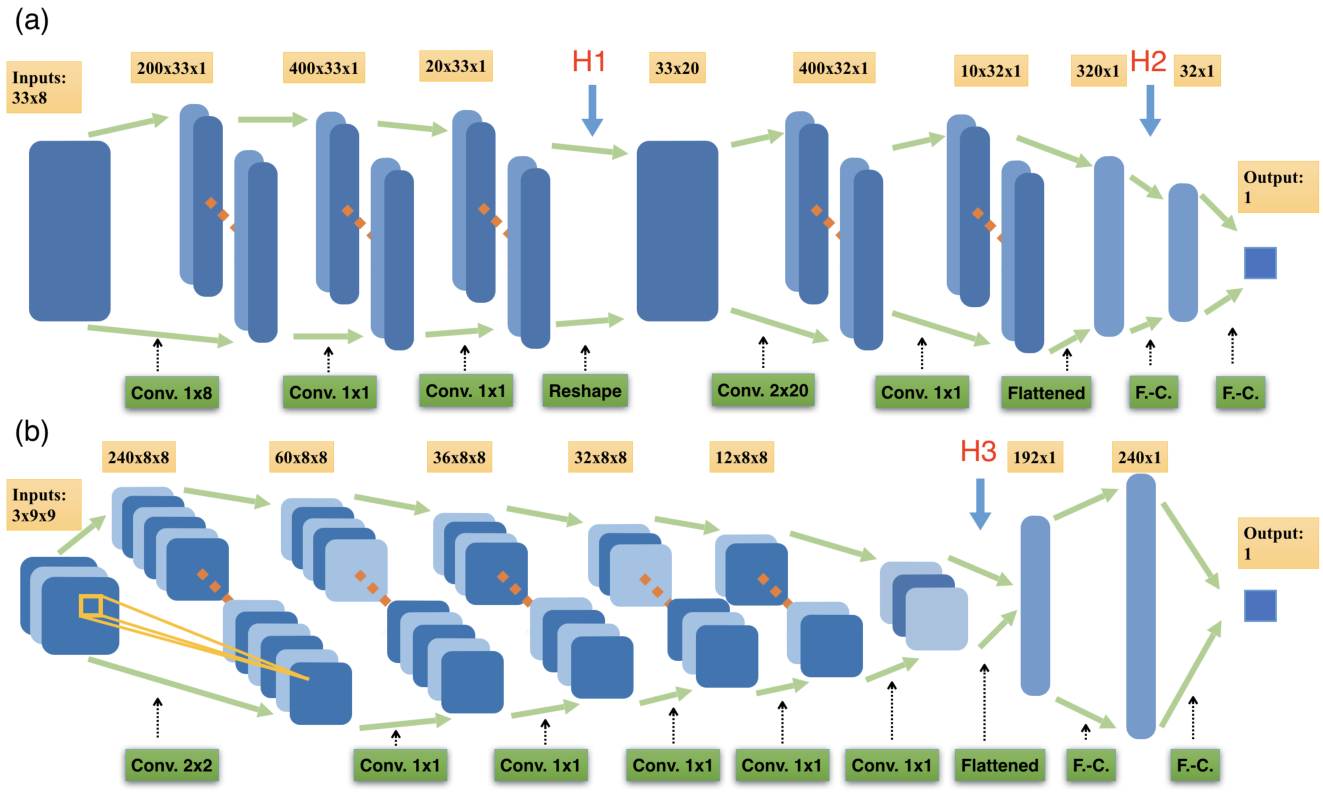
\includegraphics[width=1.0\columnwidth]{topoml/architecture}
\caption{深度学习拓扑物态网络结构示意图。(a) 训练学习一维 AIII 类绕数的网络结构;(b) 训练学习二维 A 类 Chern 数的网络结构。网络结构左侧为输入数据,右侧为输出标签。图中每一列上面标注了该层网络的神经元数目,其中左侧第一栏为输入数据的大小。层与层之间的箭头下方标注了该连接为全连接(Fully-Connected,F.-C.)还是卷积连接(Convolution,Conv.)。其中,卷积连接的方式标注了卷积核(kernel)的数目。(a) 中的两个箭头所指的地方,H1 和 H2,以及 (b) 中箭头所指的地方,H3,标注了三个隐藏层,这些隐藏层在机器训练好后的测试中被发现提取到了关键的局域特征和全局信息。其中 (a) 中的隐藏层 H1 和 H2 提取到了\textit{转角} (winding angle)的特征(见图\ref{fig:anal-winding}),(a) 中的隐藏层 H3 被发现提取到了 \textit{固体角}(solid angle),也即 Berry 曲率的特征(见图\ref{fig:anal-chern})。这对理解机器学习方法的黑匣子,与理解机器经过训练之后具有的推广预言能力来说至关重要。(取自\inlinecite{topoml})}
\label{fig:architecture}
\end{figure}




\subsection{一维 AIII 类 绕数的学习}
这一小节我们讨论一维 AIII 类拓扑类的机器学习问题。由 \ref{sec:classify} 节所述,哈密顿量矩阵为
\begin{align}\label{eq:D(k)}
    H(k)=\begin{pmatrix} 0 & D(k) \\ D^{\dagger}(k) & 0 \end{pmatrix}.
\end{align}
其中 $k$ 为U(1) 的参数。不失一般性地,我们这里选择 $D(k)$ 为幺正矩阵\footnote{平带近似不影响拓扑数,只要保持能隙不关闭就好。下同。}。由 \ref{sec:classify} 所述,这一类模型的拓扑由如下定义的绕数所刻画
\begin{align}
    w=\frac{1}{2\pi}\int_{-\pi}^{\pi}dk\mathrm{Tr}[D^{-1}(k)i\partial_kD(k)]. \label{wd1}
\end{align}
这里,由于 $D(k)$ 为幺正矩阵,其可被对角化为
\begin{align}
D(k) = V^\dag(k)M(k)V(k)
\end{align}
其中 $M(k)$ 为对角矩阵,且矩阵元全部为模1的复数,$\{e^{-i\theta_1(k)}, e^{-i\theta_2(k)},...,e^{-i\theta_d(k)}\}$。事实上,$D(k)$ 总是可以被分解为
\begin{align}
D(k) = e^{-\ii\alpha(k)}\bar{D}(k)
\end{align}
其中 $\bar{D}(k)$ 为 SU(d) 矩阵,$d$ 为矩阵维度,而
\begin{align}
\alpha(k)=\sum_i\theta_i(k)/d\in [-\pi/d,\pi/d)
\end{align}
这样以来,绕数公式可以继续被简化,
\begin{align}\label{eq:wdalpha}
    w=\dfrac{1}{\pi}\int_{-\pi}^{\pi}dk\partial_k\alpha(k),
\end{align}
在我们的工作中\cite{topoml},我们考虑 $d=2$ 的情况。这种情况下有
\begin{align}
\alpha(k)=(\theta_1(k)+\theta_2(k))/2 \mod \pi
\end{align}
而
\begin{align}
\alpha(k)\in[-\pi/2,\pi/2)
\end{align}
因此,将参数 $k$ 做离散化后,上述绕数公式在离散化的版本下写作
\begin{align}
    w &=\dfrac{1}{\pi}\sum_{l=1}^{L}\Delta\alpha(k_l) \notag\\
        &=\dfrac{1}{\pi}\sum_{l=1}^{L}[\alpha(k_{l+1})-\alpha(k_l)]\mod \pi, \label{wd_dis}
\end{align}
这里 $ k_i $, $ i=1,\ldots,L $ 均匀分布在第一布里渊区,且有
\begin{align}
\Delta\alpha(k)\in[-\pi/2,\pi/2)
\end{align}

\begin{figure}[!htb]
\centering
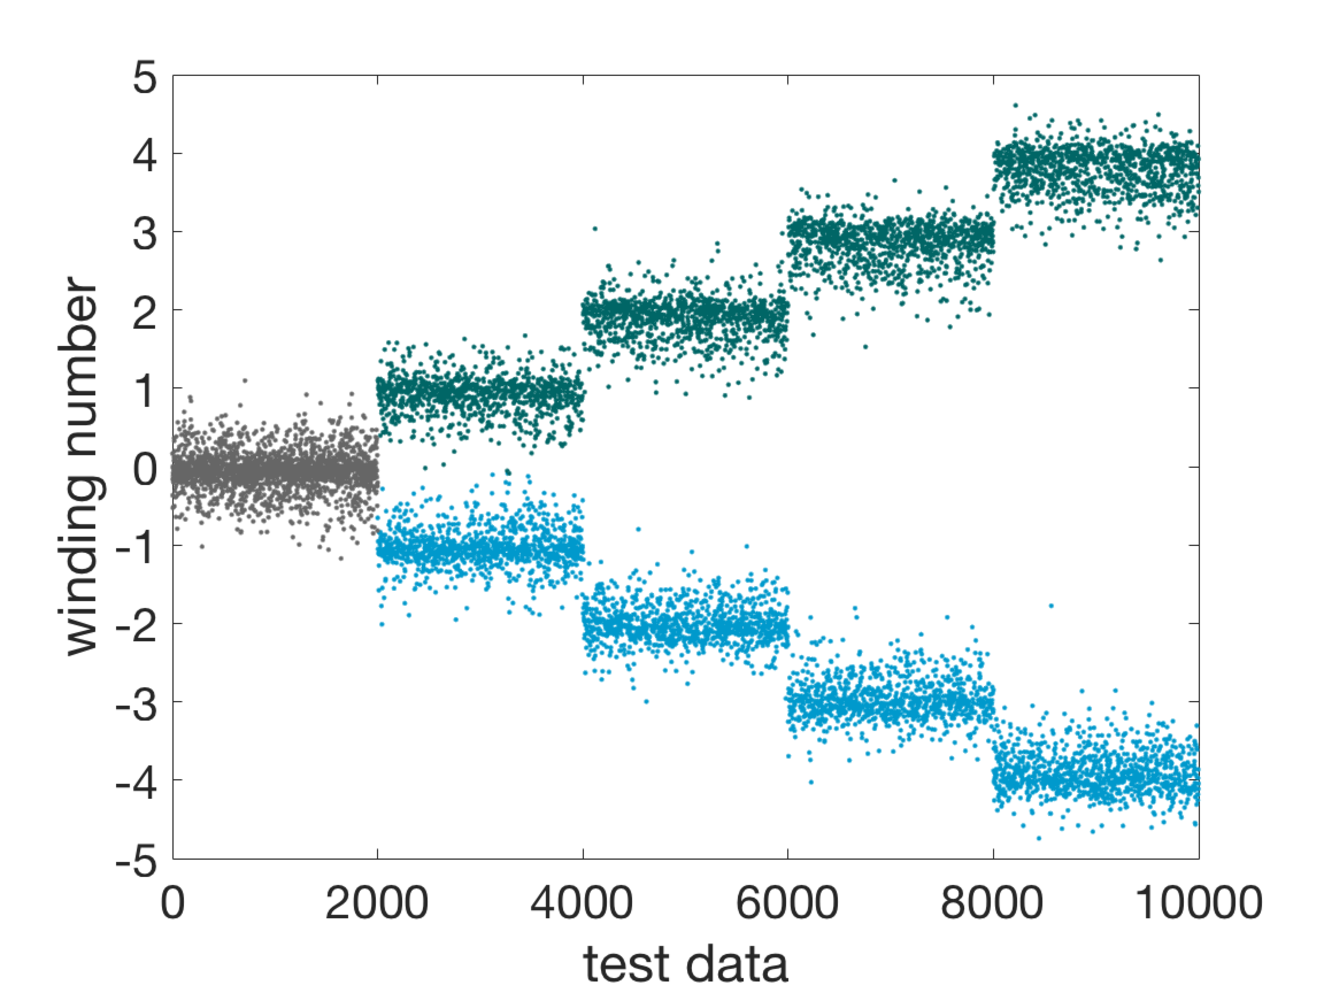
\includegraphics[width=1.0\columnwidth]{topoml/winding_performance}
\caption{一维绕数的测试表现结果。测试在10000组哈密顿量构型上进行,它们分别被标记为1到10000,即横坐标。注意,这里的标记并不是训练的标签,而是指图中的横坐标,图 \ref{fig:perf-chern} 中同此。
其中,从2000 i到2000(i+1)的哈密顿量具有$\pm i$的绕数,其中 $+$ 的以绿色标记,$-$的以青色标记。图中点的纵坐标即测试中机器所预言的结果(神经网络\ref{fig:architecture}(a)的输出)。(取自\inlinecite{topoml})}
\label{fig:perf-winding}
\end{figure}

我们对这一类模型的绕数进行了监督式学习,利用了深层的卷积神经网络,网络结构如图 \ref{fig:architecture} (a) 所示。
其用来训练的输入数据是哈密顿量构型,标签为模型的绕数。模型构型即如下矩阵
\begin{align}
    \begin{pmatrix}
        \Re[D_{11}(0)] & \Re[D_{11}(2\pi/L)] & \cdots & \Re[D_{11}(2\pi)] \\
        \Im[D_{11}(0)] & \Im[D_{11}(2\pi/L)] & \cdots & \Im[D_{11}(2\pi)] \\
        \Re[D_{12}(0)] & \Re[D_{12}(2\pi/L)] & \cdots & \Re[D_{12}(2\pi)] \\
        \Im[D_{12}(0)] & \Im[D_{12}(2\pi/L)] & \cdots & \Im[D_{12}(2\pi)] \\
        \Re[D_{21}(0)] & \Re[D_{21}(2\pi/L)] & \cdots & \Re[D_{21}(2\pi)] \\
        \Im[D_{21}(0)] & \Im[D_{21}(2\pi/L)] & \cdots & \Im[D_{21}(2\pi)] \\
        \Re[D_{22}(0)] & \Re[D_{22}(2\pi/L)] & \cdots & \Re[D_{22}(2\pi)] \\
        \Im[D_{22}(0)] & \Im[D_{22}(2\pi/L)] & \cdots & \Im[D_{22}(2\pi)]
    \end{pmatrix}
\end{align}
其中 $\Re$ 表示复数的实部,$\Im$ 表示复数的虚部。这是一个 $8\times L$ 的矩阵。当离散化到 $L=32$ 时,即 $8\times32$ 的矩阵,如图 \ref{fig:architecture}(a) 所示。
\footnote{图 \ref{fig:architecture}(a) 中 input 显示 $33\times8$,实际上是考虑了周期性边界条件,把第一列输入在最后一列后面复制了一遍。在下面的二维Chern数的例子里,也是如此。}

我们用 python TensorFlow 库 和 Wolfram Mathematica 写程序实现上述机器学习任务。训练集里的模型哈密顿量具有$\{0, \pm1, \pm2, \pm3\}$的绕数。经训练后的网络在测试集上的表现如表\ref{table:winding-sr}所示。
\footnote{具体训练和测试参数见我们的文章\inlinecite{topoml}。}
\begin{table}[t]
\caption{神经网络在测试集上的表现。对于绕数(w)分别为 $0, \pm1, \pm2, \pm3, \pm4$ 的测试哈密顿量,神经网络 \ref{fig:architecture} (a) 输出结果的正确率。 }\label{table:winding-sr}
\centering
% \begin{ruledtabular}
\begin{tabular}{*{8}c}
\hline\hline
& 绕数(w) & 0 & $\pm1$ & $\pm2$ & $\pm3$ & $\pm4$ & \\ \hline
& 正确率 & 97\% & 96\% & 96\% & 95\% & 93\% & \\
\hline\hline
\end{tabular}
% \end{ruledtabular}
\end{table}
其在测试集上的表现如图 \ref{fig:perf-winding} 所示。
可见,经训练后的神经网络在测试集上的测试结果具有很高精确度,对于已见过的类能以$>95\%$的精确度进行预言,甚至还可以以 $>90\%$ 的精确度预言绕数为 $\pm4$ 的类,具有一定程度的推广能力。




\begin{figure}[t]
\centering
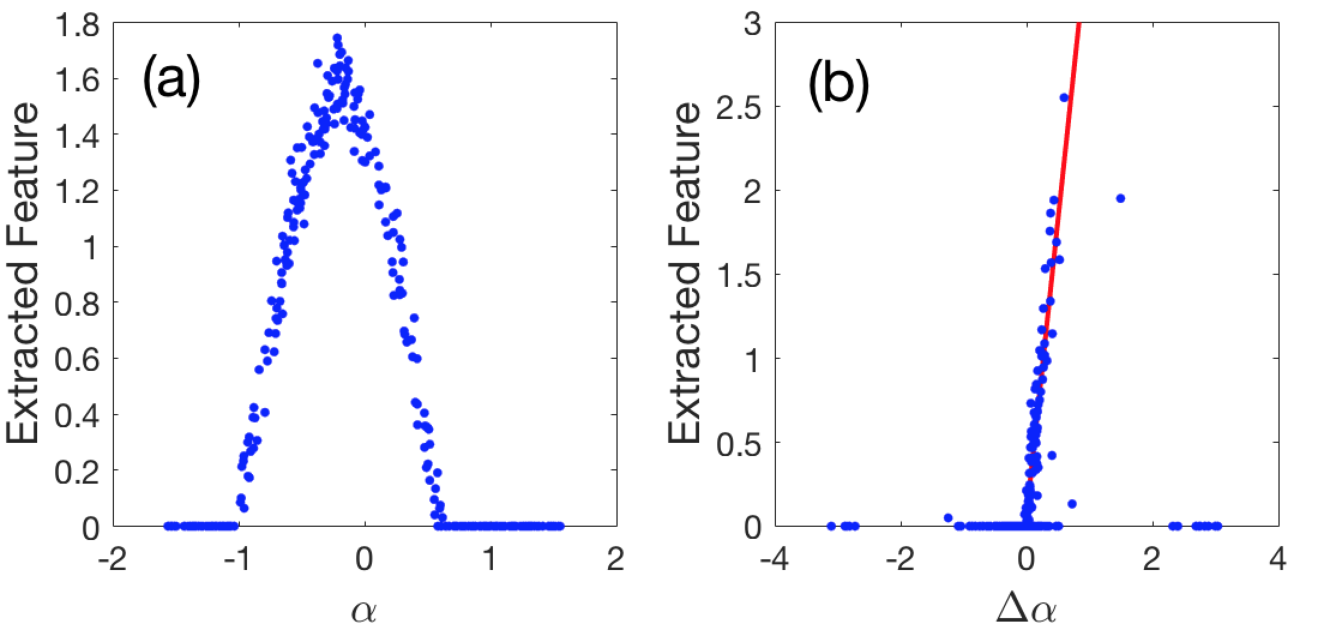
\includegraphics[width=1.0\columnwidth]{topoml/analysis_winding}
\caption{一维绕数学习的神经网络结构隐藏层分析。在机器完成训练后之后进行测试,打开神经网络\ref{fig:architecture}(a),其中的隐藏层H1 和 H2 的中间输出结果。(a) H1层的输出结果散点图,横坐标为测试模型的 $\alpha$ 角的真实值,而纵坐标为 H1 层 的输出结果,可见 H1 层实际上提取到了模型的 $\alpha$ 特征;(b) H2层输出结果的散点图,横坐标为测试模型的 $\Delta\alpha$ 的真实值,而纵坐标为 H2层的输出结果,可见 H2 层实际上提取到了模型的 $\Delta\alpha$ 特征。(取自\inlinecite{topoml})}
\label{fig:anal-winding}
\end{figure}



为理解神经网络进行绕数学习的黑盒子,以及理解其训练后具有推广能力的原因,我们尝试对训练后的神经网络结构进行解析。通过打开图 \ref{fig:architecture} (a) 中的网络,查看其隐藏层的输出,我们一定程度上理解了其学习机理。如图 \ref{fig:anal-winding} (a) 所示,通过画出 $\alpha$ 角和 H1 输出值的散点图,可以看出,H1 层实际上提取到了 $\alpha$ 角的有效特征。而如图 \ref{fig:anal-winding} (b) 所示,通过画出 $\Delta\alpha$ 和 H2 输出值的散点图,可以看出,H2 层实际上提取到了 $\Delta\alpha$ 的有效特征。而根据(\ref{eq:wdalpha})和(\ref{wd_dis})式,绕数实际上正是由 $\alpha$ 和 $\Delta\alpha$ 所计算出。这也就说明,机器通过提取到模型局部的几何特征和全局的拓扑信息、学习物理的规律而学会了绕数,而不是蒙上的。这也正是其推广能力的来源。这在下面的 Chern 数的机器学习中也能体现出来。




\subsection{二维 A 类 陈数的学习}
这一小节我们讨论二维 A 类拓扑类的机器学习问题。由 \ref{sec:classify} 节所述,A 类没有对称性约束。在此我们考虑两能带模型,对这样的模型,哈密顿量矩阵可以一般地写为:
\begin{align}
    H(\mathbf{k})=\mathbf{h}(\mathbf{k})\cdot\boldsymbol{\sigma}=h_x(\mathbf{k})\sigma_x+h_y(\mathbf{k})\sigma_y+h_z(\mathbf{k})\sigma_z.
\end{align}
这里 $\boldsymbol{\sigma}=(\sigma_x,\sigma_y,\sigma_z)$ 是泡利矩阵矢量,和上一小节一样,我们取平带近似,这不影响其拓扑刻画。对于二维模型,其拓扑由下式 Chern 数刻画,
\begin{align}\label{eq:c1}
    C=\dfrac{1}{2\pi}\int_{T^2}d^2\mathbf{k}F_{xy}(\mathbf{k}), 
\end{align}
这里 $T^2$ 指第一布里渊区(Torus结构),而
\begin{align}%\label{eq:c1AF}
A_{\mu}(\mathbf{k}) &= i\langle u(\mathbf{k})|\partial_{\mu} u(\mathbf{k})\rangle, \\ 
F_{\mu\nu}(\mathbf{k}) &= \partial_{\mu}A_{\nu}-\partial_{\nu}A_{\mu}.
\end{align}

\begin{figure}[t]
\centering
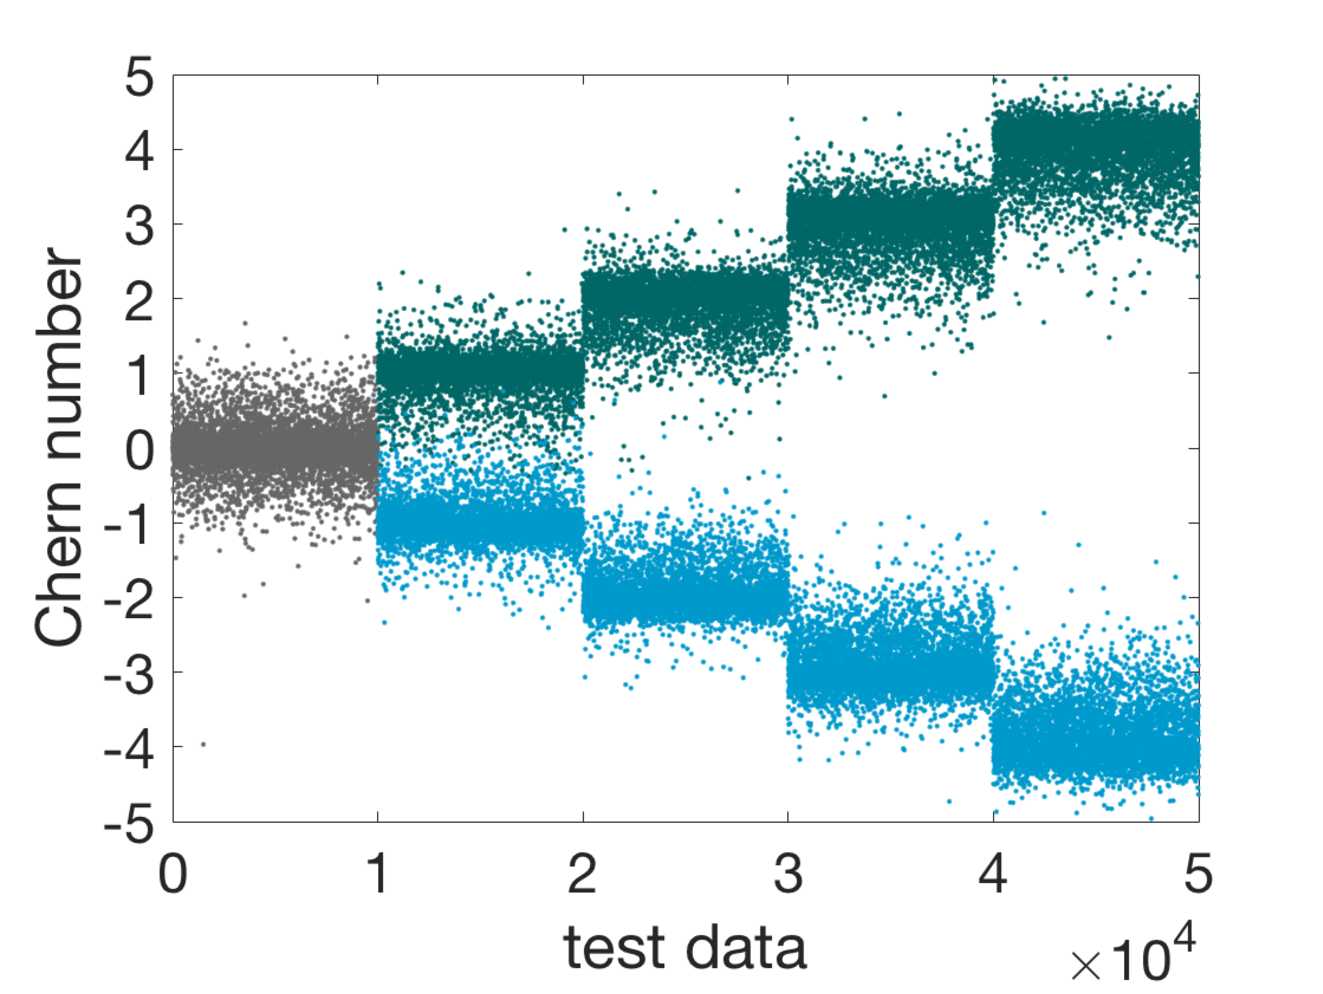
\includegraphics[width=1.0\columnwidth]{topoml/chern_performance}
\caption{二维Chern数的学习测试表现结果。测试在 $5\times10^4$ 组哈密顿量构型上进行,它们分别被标记为1到50000,即横坐标的值。其中,从10000i 到10000(i+1)的哈密顿量具有 $\pm i$ 的Chern 数,其中 $+$ 的以绿色标记,$-$的以青色标记。图中点的纵坐标即测试中机器所预言的结果(神经网络\ref{fig:architecture}(b)的输出)。(取自\inlinecite{topoml})}
\label{fig:perf-chern}
\end{figure}


我们利用深层神经网络对二维 A 类两能带模型的 Chern 数进行了机器学习,网络结构如图 \ref{fig:architecture} (b) 所示。
输入数据依然为哈密顿量构型,即 
\begin{align}
\begin{pmatrix}\mathcal{H}_x, & \mathcal{H}_y, & \mathcal{H}_z 
\end{pmatrix}
\end{align}
其中
\begin{align}
\mathcal{H}_{\mu} &=
\begin{pmatrix}
h_{\mu}(0,0) & h_{\mu}(0,\frac{2\pi}{L}) & \cdots & h_{\mu}(0,2\pi) \\
h_{\mu}(\frac{2\pi}{L},0) & h_{\mu}(\frac{2\pi}{L},\frac{2\pi}{L}) & \cdots & h_{\mu}(\frac{2\pi}{L},2\pi) \\
\vdots & \vdots & \ddots & \vdots \\
h_{\mu}(2\pi,0) & h_{\mu}(2\pi,\frac{2\pi}{L}) & \cdots & h_{\mu}(2\pi,2\pi) \\
\end{pmatrix}.
\end{align}
这里将 二维参数空间 $(k_x,k_y)$ 离散化为 $L\times L$ 个格点,模型的理论 Chern 数值可有附录 \ref{sec:chern} 中的算法计算。


我们用 Wolfram Mathematica 写程序实现上述机器学习任务。训练集里的模型哈密顿量 Chern 数有 $C\in\{0, \pm1, \pm2\}$,经训练后的网络在测试集上的表现如表\ref{table:winding-sr}所示。
\footnote{具体训练和测试参数见我们的文章\inlinecite{topoml}。}

\begin{table}[t]
\centering
\caption{神经网络在测试集上的表现。对于 Chern 数分别为 $0, \pm1, \pm2, \pm3, \pm4$ 的测试哈密顿量,神经网络 \ref{fig:architecture} (b) 输出结果的正确率。}
\label{table:chern-sr}
% \begin{ruledtabular}
\begin{tabular}{*{8}c}
\hline\hline
& 陈数($C$) & $0$ & $\pm1$ & $\pm2$ & $\pm3$ & $\pm4$ & \\ \hline
& 正确率 & 93\% & 92\% & 90\% & 86\% & 85\% & \\
\hline\hline
\end{tabular}
% \end{ruledtabular}
\end{table}

其在测试集上的表现如图 \ref{fig:perf-chern} 所示。
可见,经训练后的神经网络在测试集上的测试结果具有很高精确度,对于已见过的类能以$>90\%$的精确度进行预言,甚至还可以以 $>85\%$ 的精确度预言其没有见过的 Chern 数为 $\pm3,\pm4$ 的类,具有一定程度的推广预言能力。


\begin{figure}[!htb]
\centering
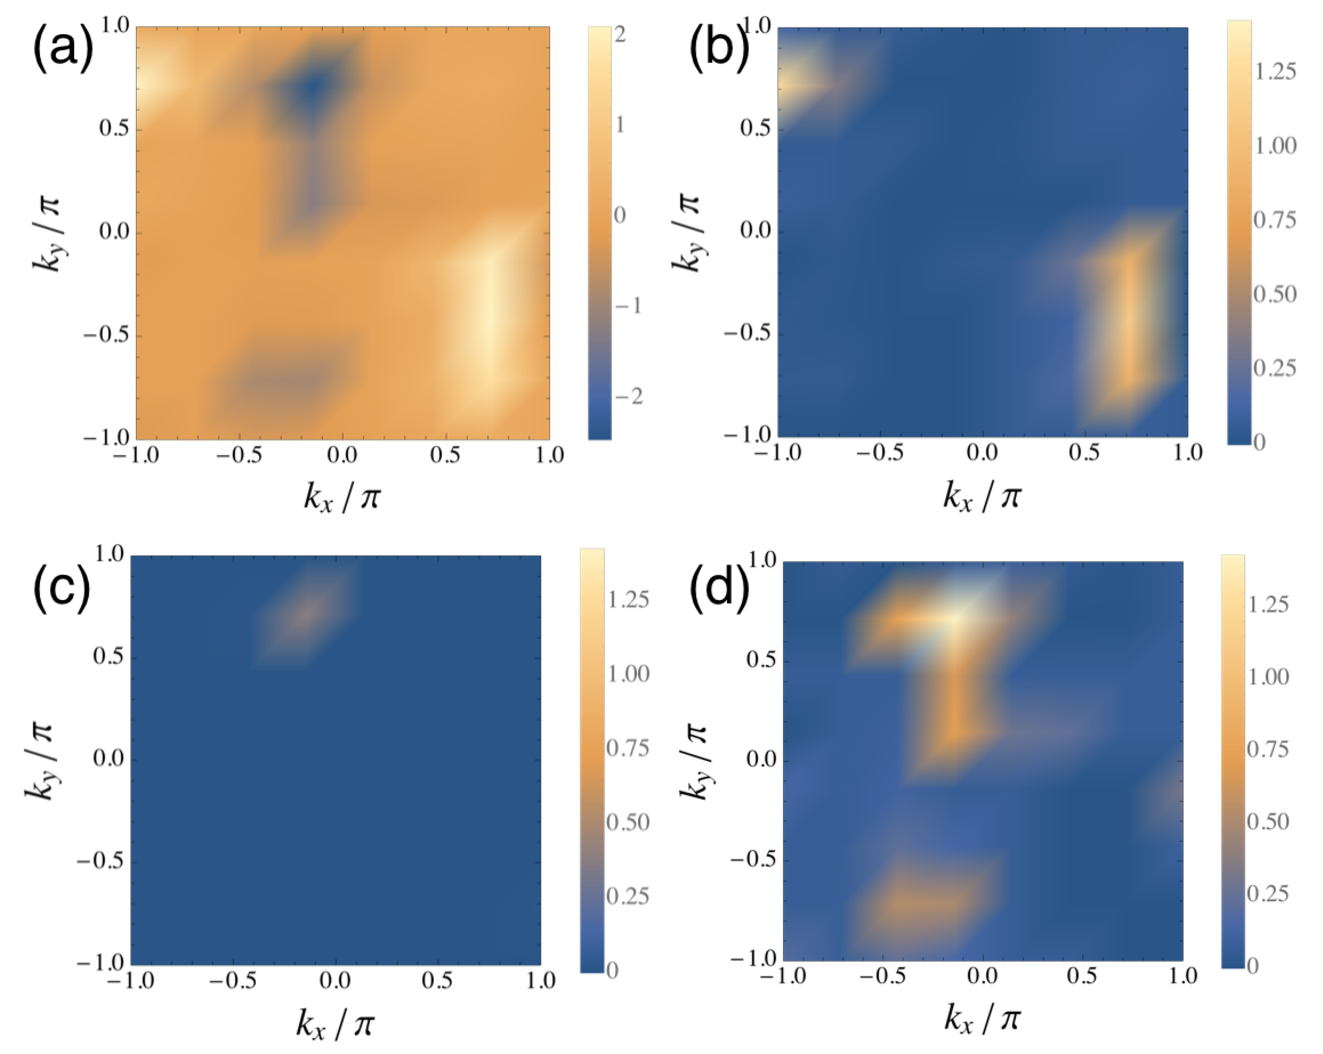
\includegraphics[width=1.0\columnwidth]{topoml/analysis_Berry}
\caption{二维Chern数学习的神经网络结构隐藏层分析。在机器完成训练之后进行测试,打开神经网络\ref{fig:architecture}(b),其中的隐藏层 H3 的中间输出结果。注意到,H3为三层的矩阵输出。(a) 测试模型的 Berry 曲率场真实值,由附录\ref{sec:chern} 中所述算法算得;对比图例可以看到,其中矩阵元有正有负。(b-d) H3 处三层矩阵的输出值;对比图例可以看出,输出值均为正值,且 (b) 层主要提取到了 (a) 中的正的部分,(d) 层主要提取到了 (a) 中的负的部分,而 (c) 层神经元几乎全部死掉(输出为0)。可见,H3 层实际上提取到了模型的 Berry 曲率场(也就是固体角)特征。(取自\inlinecite{topoml})}
\label{fig:anal-chern}
\end{figure}

为理解其学习机理和推广能力,我们将神经网络内层打开,尝试解析训练后的神经网络结构。如图 \ref{fig:architecture}(b) 所示,我们领网络在 H3 处输出其中间结果,对某一个典型的例子的输出结果如图 \ref{fig:anal-chern} 所示。其中,图 \ref{fig:anal-chern} (a) 为该模型的真实的 Berry 曲率场,而 (b-d) 为 H3 的输出结果。(a) 的值有正有负,而 (b-d) 均为正值,对比图例可知。这与神经网络中所取的激活元为 ReLU 函数有密切关系\cite{topoml}。由图还可看出,(c) 中的神经元大多死掉了,而 (b) 和 (d) 则通过分别提取 (a) 中正的部分和负的部分来提取到了 Berry 曲率场的全局特征。

由此可见,对神经网络进行拓扑数的训练使其学到了不止是拓扑数一个数字,而是有效地提取到模型局部的几何特征和全局的拓扑信息,物理的特征被包括其中。我们在训练的时候,并没有告诉机器要去学习积分公式或者几何相角这样的局域信息,只是扔给它一个拓扑数的标签,而经过训练,机器自己学会了提取局域的几何特征和全局的拓扑特征。这也是其具有推广预言能力的来源。这使我们对机器的学习机理有了一定程度的理解。

这里需要补充说明的是,我们生成模型的方式是通过随机生成模型的傅立叶分量来构造大量的模型,这些模型构型随后被用于机器的训练或测试。这个过程中并没有检测这些模型是不是一定有能隙的,或者对于离散化的模型,其能隙可能是非常小,以致于 Berry 曲率会非常奇异。然而,无能隙的体系是不能算其 Chern 数的,对于离散化的情况,Berry 曲率过去奇异也会导致计算结果有偏差(见附录\ref{sec:chern}讨论)。事实上,这可能正是上述机器语言精确度没有达到很精确\footnote{很精确,例如99\%,99.9\%, 甚至更高}的原因之一。当然,这种偏差可以通过增加足够大的离散化来减小,而这又会使输入数据的维度大大增大,使机器训练的难度变大。当数据数据的维度增大很多时,网络结构本身可能就需要重新设计了。



